% Chapter 1
\addchap{Introduction}
\label{chapter-introduction} 
%----------------------------------------------------------------------------------------
% Define some commands to keep the formatting separated from the content 
\newcommand{\keyword}[1]{\textbf{#1}}
\newcommand{\tabhead}[1]{\textbf{#1}}
\newcommand{\code}[1]{\texttt{#1}}
\newcommand{\file}[1]{\texttt{\bfseries#1}}
\newcommand{\option}[1]{\texttt{\itshape#1}}
%----------------------------------------------------------------------------------------
\section*{Importance of the topic}
\addcontentsline{toc}{section}{Importance of the topic}  
The desire for an integrated information system serving the needs of the biodiversity community dates at least as far back as 1985 when the Taxonomy Database Working Group (TDWG)---later renamed to Biodiversity Informatics Standards but retaining the abbreviation TDWG---was established\footnote{A webpage with the history of TDWG dating back to 1985 can be viewed under \url{http://old.tdwg.org/past-meetings/}; however, a lot of the links are unfortunately broken and the page needs some maintenance.}. In 1999, the Global Biodiversity Information Facility (GBIF) was created after the Organization for Economic Cooperation and Development (OECD) had arrived at the conclusion that \emph{``an international mechanism is needed to make biodiversity data and information accessible worldwide''} (\cite{noauthor_what_nodate}).  The Bouchout declaration (\cite{noauthor_bouchout_2014}) crowned the results of the European Union--funded project \cite{noauthor_pro-ibiosphere_nodate} that lasted from 2012 to 2014 and was dedicated to the task of creating an integrated biodiversity information system. The Bouchout declaration proposes to make scholarly biodiversity knowledge freely available as Linked Open Data (LOD).  A parallel process in the U.S.A. started even earlier with the establishment of the Global Names Architecture, GNA (\cite{patterson_names_2010,pyle_towards_2016}).

In 2014, the Horizon 2020 BIG4 consortium was formed between academia and industry dedicated to advancing biodiversity science.  The project's mission statement reads \emph{``BIG4---Biosystematics, Informatics and Genetics of the big 4 insect groups: training tomorrow's researchers and entrepreneurs''} (\cite{university_of_copenhagen_big4_2014}). An important member of the consortium is the academic publishing house and software company, Pensoft Publishers. It publishes several dozen well-known open access taxonomic journals\footnote{For example, ZooKeys, PhytoKeys, MycoKeys, and Biodiversity Data Journal (BDJ).} and, as a signatory of the Bouchout declaration, was a prime candidate to push the vision for an Open Biodiversity Knowledge Management System (OBKMS) forward. The presented Ph.D. project is based at Pensoft Publishers and at the Institute of Information and Communication Technology (IICT) of the Bulgarian Academy of Sciences with the goal to follow through pro-iBiosphere's vision.

\section*{Previous work}
\addcontentsline{toc}{section}{Previous work}

Due to the interdisciplinary nature of the thesis, this section will focus on two areas: (a) knowledge bases and Linked Open Data and (b) biodiversity publishing.

\subsection*{Knowledge bases and Linked Open Data}
\addcontentsline{toc}{subsection}{Knowledge bases and Linked Open Data}

We shall start by first introducing \emph{knowledge bases} and \emph{knowledge-based systems}.  We use the two terms interchangeably but tend to write the longer variant, knowledge-based system, when we want to emphasize aspects of the knowledge base that are not related to the underlying facts store (database).

It is useful to form one's concept of knowledge-based systems both by looking at explicit definitions and by looking at several examples of knowledge bases in practice. The term was already being widely discussed by the 1980's (\cite{brodie_kbms_1989}) and early nineties (\cite{harris_knowledge_1993}) and was understood to mean the utilization of ideas from both database management systems (DBMS) and artificial intelligence (AI) to create a type of computer system called \emph{knowledge base management system} (KBMS). \cite{harris_knowledge_1993} writes that the characteristics of a knowledge base management system are that it contains \emph{``prestored rules and facts from which useful inferences and conclusions may be drawn by an inference engine.''}  We should note that the phrase ``prestored rules'' comes from the time of first-generation AI systems that were rule-based. Recently, there has been progress in incorporating statistical techniques into databases (\cite{mansinghka_bayesdb:_2015}); however, in this project we are working with the classical rule-based definition. In other words, a knowledge base is, in our understanding, \emph{a suitable database tightly integrated with a logic layer.}

Another relatively recent development in knowledge-based systems has been the application of the Linked Data principles (\cite{heath_linked_2011}). In fact, most existing knowledge bases emphasize the community aspects of making data more interconnected and reusable. Examples include Freebase (\cite{bollacker_freebase:_2008}), which was recently incorporated in WikiData (\cite{vrandecic_wikidata:_2014, pellissier_tanon_freebase_2016}), DBPedia (\cite{hutchison_dbpedia:_2007}), as well as Wolfram|Alpha (\cite{noauthor_wolfram|alpha_nodate}) and the Google Knowledge Graph (\cite{singhal_introducing_2012}). What these systems have in common is that an emphasis is placed not only on the logic layer allowing inference but on a unified information space: these systems act as nexus integrating information from multiple places and they follow to various degrees the principles of Linked Open Data (LOD).

Linked Open Data (\cite{heath_linked_2011}) is a concept of the Semantic Web (\cite{berners-lee_semantic_2001}), which, when applied properly, ensures that data published on the Web is reusable, discoverable, and most importantly ensures that pieces of data published by different entities can work together.  We will discuss the Linked Data principles and their application to OpenBiodiv in detail in Chapter~\ref{chapter-lod}.

Leveraging these developments, modern knowledge bases place a bigger emphasis on interlinking data rather than on developing a complex inference machinery. There has been critique of the idea of bundling logic in the database layer as such bundling leads to increased complexity (\cite{barrasa_rdf_2017}). The critique can be summarized with two points. First, bundling the logic near the data (especially when it is excessive for the task at hand) can lead to drastic performance decreases\footnote{ We will compare the performance of the stronger Web Ontology Language (OWL) logic layer with a weaker RDF Schema (RDFS) logic layer in Chapter~\ref{chapter-lod}. Resource Description Framework (RDF) is a data model for storing statements about things discussed later.}. Second, the developing of new techniques (e.g. machine learning) can make the existing deep logic layer obsolete. Our view is that data is the commodity which is much more valuable, and the inference strategy (be it a rule-based logic layer, or a statistical machine learning technique) can be replaced as computational science moves forward. These ideas lead to an interesting conundrum in the choice of a database technology discussed in the subsequent sections.

Finally, a knowledge-based system ultimately needs to include user-interface components (UI's) and application programming interfaces (API's) or an application layer. These serve as the point-of-contact for human-computer, or computer-computer interaction, and are crucial to the success of any such system.

\subsection*{Biodiversity publishing}
\addcontentsline{toc}{subsection}{Biodiversity publishing}

In the biomedical domain there are well-established efforts to extract information and discover knowledge from literature (e.g. \cite{rebholz-schuhmann_facts_2005, momtchev_expanding_2009, williams_open_2012}).  The biodiversity domain, and in particular biological systematics and taxonomy (from here on in this thesis referred to as \emph{taxonomy}), is also moving in the direction of semantization of its research outputs (\cite{agosti_biodiversity_2006, patterson_taxonomic_2006,kennedy_scientific_2005,penev_fast_2010, tzitzikas_integrating_2013}).  The publishing domain has been modeled through the Semantic Publishing and Referencing Ontologies, SPAR Ontologies (\cite{peroni_semantic_2014}).   The SPAR Ontologies are a collection of ontologies incorporating, amongst others, FaBiO, the FRBR-aligned Bibliographic Ontology (\cite{peroni_fabio_2012}), and DoCO, the Document Component Ontology (\cite{constantin_document_2016}).   The SPAR Ontologies provide a set of classes and properties for the description of general-purpose journal articles, their components, and related publishing resources.  Taxonomic articles and their components, on the other hand, have been modeled through the TaxPub XML Document Type Definition (DTD)---also referred to loosely as XML schema---and the Treatment Ontologies (\cite{catapano_taxpub:_2010}).  While TaxPub is the XML-schema of taxonomic publishing for several important taxonomic journals (e.g. ZooKeys, PhytoKeys, Biodiversity Data Journal), the Treatment Ontologies are still in development and have served as a conceptual template for OpenBiodiv-O (discussed in Chapter~\ref{chapter-ontology}). 

Taxonomic nomenclature is a discipline with a very long tradition.  It transitioned to its modern form with the publication of the Linnaean System (\cite{linnaeus_systema_1758}).  Already by the beginning of the last century, there were hundreds of taxonomic terms in usage (\cite{witteveen_naming_2015}).  At present the naming of organismal groups is governed by the International Code of Zoological Nomenclature, ICZN (\cite{international_commission_on_zoological_nomenclature_international_1999}) and by the International Code of Nomenclature for algae, fungi, and plants, Melbourne Code (\cite{noauthor_international_2012}).  Due to their complexity (e.g. ICZN has 18 chapters and 3 appendices), it proved challenging to create a top-down ontology of biological nomenclature. Example attempts include the relatively complete NOMEN ontology (\cite{dmitriev_nomen_2017}) and the somewhat less complete Taxonomic Nomenclatural Status Terms, TNSS\footnote{Even though it is unknown to the authors whether TNSS was published in peer-reviewed literature, remnants of it can still be found on GitHub, e.g. under \url{https://github.com/pensoft/OpenBiodiv/blob/master/ontology/contrib/taxonomic_nomenclatural_status_terms.owl}.}.

There are several projects that are aimed at modeling the broader biodiversity domain conceptually. Darwin Semantic Web, Darwin-SW (\cite{baskauf_darwin-sw:_2016}) adapts the previously existing Darwin Core (DwC) terms (\cite{wieczorek_darwin_2012}) as RDF (\cite{rdf_working_group_resource_2014}). These models deal primarily with organismal occurrence data.

Modeling and formalization of the strictly taxonomic domain has been discussed by Berendsohn (\cite{berendsohn_concept_1995}) and later, e.g., in (\cite{franz_perspectives:_2009,sterner_taxonomy_2017}). Noteworthy efforts are the XML-based Taxonomic Concept Transfer Schema (\cite{taxonomic_names_and_concepts_interest_group_taxonomic_2006}) and a now defunct Taxon Concept ontology. Very recently, the TDWG community has attempted to resurrect the Taxon Concept ontology with the Taxonomic Names and Concepts Interest Group. The group discussions can be accessed under \url{https://github.com/tdwg/tnc}. Interestingly the \href{https://github.com/tdwg/tnc/issues/1}{very first GitHub issue} discussed OpenBiodiv-O and the possibility of its adoption as a TDWG standard.

By the time the OpenBiodiv project started in June 2015, a number of articles had been previously published on the topics of linking data and sharing identifiers in the biodiversity knowledge space (\cite{page_biodiversity_2008}), unifying phylogenetic knowledge (\cite{parr_evolutionary_2012}), taxonomic names and their relation to the Semantic Web (\cite{page_taxonomic_2006,patterson_names_2010}), and aggregating and tagging biodiversity research (\cite{mindell_aggregating_2011}). Some partial discussion of OBKMS was to be found in the science blog \href{http://iphylo.blogspot.bg}{iPhylo} (\cite{page_vision_2014, page_putting_2015}). The legal aspects of the OBKMS had been discussed by \cite{egloff_open_2014}.

Furthermore, several tools and systems that deal with the integration of biodiversity and biodiversity data had been developed by different groups. Some of the most important ones are UBio, Global Names, BioGuid, BioNames, Pensoft Taxon Profile, and the Plazi Treatment Repository\footnote{UBio: \href{http://ubio.org/}{http://ubio.org/}; Global Names: \href{http://globalnames.org/}{http://globalnames.org/}; BioGuid: \href{http://bioguid.org/}{http://bioguid.org/}; BioNames: \href{http://bionames.org/}{http://bionames.org/}; Pensoft Taxon Profile: \href{http://ptp.pensoft.eu/}{http://ptp.pensoft.eu/}; Plazi Treatment Repository: \href{http://plazi.org/wiki/}{http://plazi.org/wiki/}.}.

\subsection*{Key findings}
\addcontentsline{toc}{subsection}{Key findings}

The key findings from the papers cited in the previous paragraphs can be summarized as follows:

\begin{enumerate}
  
\item{Biodiversity science deals with disparate types of data: taxonomic, biogeographic, phylogenetic, visual, descriptive, and others. These data are siloed in unlinked data repositories.}
  
\item{Biodiversity databases need a universal system of naming concepts due to the inefficiencies of Linnaean names for modern taxonomy. Taxonomic concept labels have been proposed as a human-readable solution and stable globally unique identifiers of taxonomic concepts had been proposed as a machine-readable solution.}

\item{There is a base of digitized semi-structured biodiversity information online with appropriate licenses waiting to be integrated as a knowledge base.}
\end{enumerate}


\section*{Goal and objectives}
\addcontentsline{toc}{section}{Goal and objectives}

Given the huge international interest in an open biodiversity knowledge management system (OBKMS), this dissertation started the OpenBiodiv project, the goal of which is to contribute to OBKMS by focusing on biodiversity information extracted from scholarly literature. The scientific goal of the project is to create a formal semantic model of the domain of biodiversity publishing and to apply this model for the creation of a Linked Open Dataset from biodiversity data.

\paragraph{Objective 1: Ontology.} Study the domain of biodiversity informatics and biodiversity publishing and develop an ontology allowing data integration from diverse sources.

\paragraph{Objective 2: Software architecture.} Formally define OpenBiodiv as a knowledge-based system and design its integrated software architecture.

\paragraph{Objective 3: Linked open dataset.} Create a Linked open dataset (LOD) on the basis of published taxonomic articles using the ontology defined in Objective 1.

\paragraph{Objective 4: Library.} Develop methods for converting taxonomic publications into the semantic model of the ontology in order to support Objective 3.

\paragraph{Objective 5: Workflows.} Develop practical workflows for continuously converting taxonomic data into taxonomic publications and thus updating the LOD dataset.

\paragraph{Objective 6: Web portal.} Create a web portal and example applications on top of the knowledge base.

\section*{Methodology}
\addcontentsline{toc}{section}{Methodology}

In this section the "meta-choices" (methological choices) are outlined that have been made before the design and implementation phase. They include but are not limited to programming methodologies and database paradigms. 

\subsection*{Choice of database paradigm for OpenBiodiv}
\addcontentsline{toc}{subsection}{Choice of database paradigm for OpenBiodiv}

We specify OpenBiodiv as a knowledge-based system with a focus on structuring and inter-linking biodiversity data. Two of the possible database technologies that fit this requirement are semantic graph databases (triple stores) such as GraphDB (\cite{ontotext_graphdb_2018}) and labeled property graphs such as Neo4J (\cite{neo4j_developers_neo4j_2012}).

Semantic graph databases offer a very simple data model: every fact stored in such a database is composed as a triple of \emph{subject}, \emph{predicate}, and \emph{object}. Subjects of triples are always resource identifiers, whereas objects can be other resource identifiers or literal values (e.g. strings, numbers, etc.). Relations between resources or between resources and literals are given by the predicates (also specified as identifiers). Such links are sometimes referred to as \emph{properties}. Thus, one can visualize a directed graph whose nodes are the subjects or objects, as specified via resource identifiers or literals, and whose arcs are predicates.

Semantic graph databases have the unique feature that the logic layer is also expressed as triples stored in the database. This logic layer, known as \emph{ontology}, is not only responsible for drawing conclusions from the data (inference), but also specifies the semantics of how knowledge should be expressed.

Labeled property graphs, on the other hand, offer a freer data model by allowing the arcs of the knowledge graph to have properties as well. For example, in a labeled property graph whose nodes are two cities A and B and are connected by a property-predicate \emph{road to}, it is possible to additionally attach the value ``500 km'' to that property. Thus, we indicate that the length of the road connecting the cities is 500 km (Fig.~\ref{fig-ab}).

\begin{figure}[h!]
	\centering
	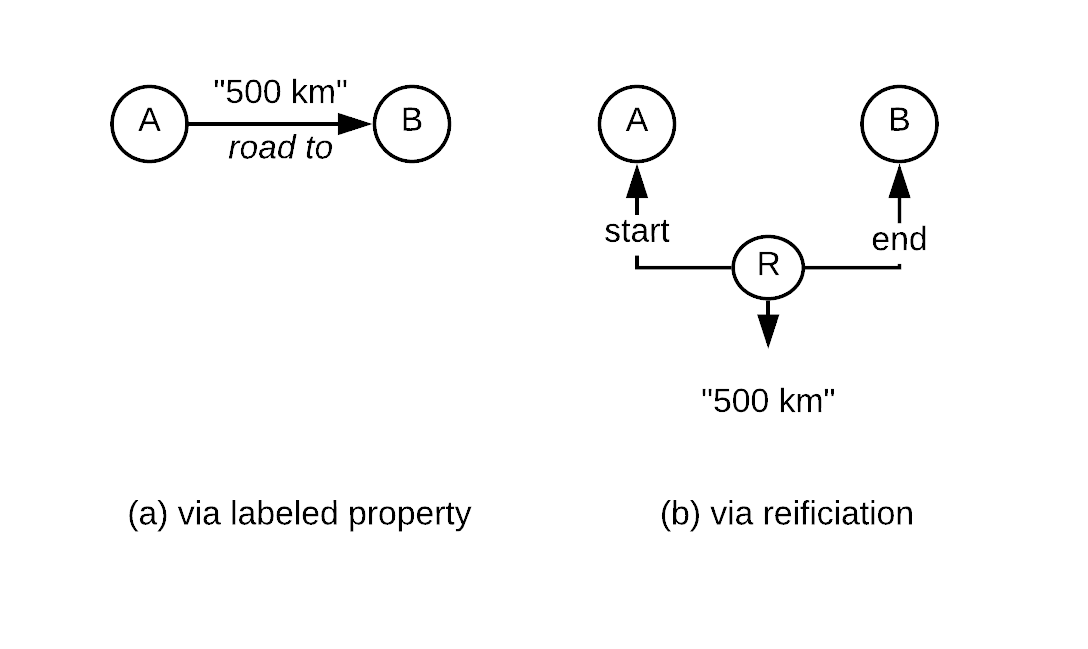
\includegraphics[width=\textwidth]{Figures/ab}
	\decoRule
  \caption{Representing the statement that two cities, $A$ and $B$, are 500 km apart via (a) a labeled property graph and via (b) reification in a semantic graph.}
  \label{fig-ab}
\end{figure}

Note that labeled property graphs are not any more expressive than what can be achieved by triples alone. In fact, complex relationships in a simple triple store can be expressed by making relationships into nodes that have properties on their own. This process is known as \emph{reification}. For example, the two cities $A$ and $B$ can connect to a further node, $R$ indicating the road. $R$ will then have three properties: \emph{start}, \emph{end}, and \emph{length}. The value (object) of \emph{start} will be $A$, of \emph{end} will be $B$, and of length will be the literal ``500 km'' (Fig.~\ref{fig-ab}).

We have summarized the differences between labeled property graphs and semantic graph databases in Table~\ref{graphdb-vs-neo4k}. After careful considerations, we settled on the triple store, i.e. semantic graph database as a choice of database technology. This decision was informed by the wide availability of high-quality ontologies and RDF data models in our domain (\cite{baskauf_darwin-sw:_2016,peroni_semantic_2014}) and the popularity of the Semantic Web (\cite{berners-lee_semantic_2001}) in the community. 

\begin{table}
\caption{Differences between semantic graph databases (e.g. GraphDB) and labeled property graphs (e.g. Neo4j).}
\begin{tabular}{>{\centering\arraybackslash}m{2.5cm}|>{\centering\arraybackslash}m{4.2cm}|>{\centering\arraybackslash}m{4.2cm}}
Criterion   & Semantic database & Labeled property graph\\
\hline
Semantics   & Stored in the database itself as OWL or RDFS statements. Provides a uniform data space. Requires expert ontologists to extract knowledge.
            & Formal semantics usually are missing. Quick deployment. Uniform data space harder to achieve.\\
\hline
Inference   & Provided by the database itself from its ontology or expressed as SPARQL queries. General purpose, slower.
            & External to the database. Needs to be written for every specific task. Special purpose. Faster.\\
\hline
Community   & Has a rich and mature community of ontologists and knowledge engineers. Lots of domain ontologies. Designed for inter-operability. Standards-driven.
            & Data models are created ad-hoc by data scientists or programmers for a particular task. Inter-operability requires effort and not of primary concern. Applications-driven.\\
\hline
\end{tabular}
\label{graphdb-vs-neo4k}
\end{table}

However, we believe that labeled property graphs are a freer and a more natural data model and are perfectly suited for biodiversity informatics. In particular they provide a much more natural formalism for relationships between taxonomic concepts (discussed in Chapter~\ref{chapter-ontology}). Also, non-RDF semantic databases such as \mbox{WikiData} are gaining in popularity. Therefore, we believe that the applicability of RDF triple stores for OpenBiodiv should constantly be reevaluated.

\subsection*{Choice of information sources}
\addcontentsline{toc}{subsection}{Choice of information sources}

According to \cite{noauthor_pro-ibiosphere_2014}, biodiversity and biodiversity-related data have two different ``life-cycles.'' In the past, after an observation of a living organism had been made, it was recorded on paper and then the observation record was published in paper-based form. In order for biodiversity data to be available to the modern scientist, efforts are made nowadays to digitize those paper-based publications by Plazi \cite{agosti_why_2007} and the Biodiversity Heritage Library (\cite{miller_taxonomic_2012}). For this purpose, several dedicated XML schemas have been developed (see \cite{penev_xml_2011} for a review), of which TaxPub (\cite{catapano_taxpub:_2010}) and TaxonX  seem to be the most widely used (\cite{penev_implementation_2012}). The digitization of publications contains several steps. After scanning and optical character recognition (OCR), text mining is combined with searching for particular kinds of data\footnote{This procedure leaves a trace in the form of marked-up (tagged) elements that can then be extracted and made available for future use and reuse (\cite{miller_integrating_2015}).}.

In present day, biodiversity data and publications are mostly ``born digital'' as semantically Enhanced Publications (EP's, \cite{claerbout_electronic_1992,godtsenhoven_van_emerging_2009,shotton_semantic_2009}). According to \cite{claerbout_electronic_1992}, \emph{``an EP is a publication that is enhanced with research data, extra materials, post publication data and database records. It has an object-based structure with explicit links between the objects. An object can be (part of) an article, a data set, an image, a movie, a comment, a module or a link to information in a database.''} Semantically enhanced publications are thus natives of the Web and the Semantic Web unlike their paper-based equivalents.

The act of publishing in a digital, enhanced format, differs from the ground up from a paper-based publication. The main difference is that a digitally-published document can be structured in such a format as to be suitable both for machine processing and to the human eye. In the field of biodiversity science, Pensoft journals such as ZooKeys, PhytoKeys, and the Biodiversity Data Journal (BDJ) already function by providing EP's (\cite{penev_semantic_2010}).

Given the fact that Pensoft Publishers' and Plazi's publications cover a large part of taxonomic literature both in volume and also in temporal span, and the fact that the publications of those two publishers are available as semantic EP's, we've chosen Pensoft's journals and Plazi's treatments as our main sources of information.

Furthermore, we incorporate the taxonomic backbone of GBIF \cite{gbif_secretariat_gbif_2017} as a source for data integration. This is further discussed in Chapter~\ref{chapter-lod}.

\subsection*{Choice of development methodology and programming environment}
\addcontentsline{toc}{subsection}{Choice of development methodology and programming environment}

In 2016, based on the outcomes of pro-iBiosphere and on the previous work in the area of biodiversity informatics, we published the Ph.D. plan for this research (\cite{senderov_open_2016}). This publication can be considered as the first design specification of OpenBiodiv. However, in the course of developing the system, its design was changed iteratively through a feedback loop from collaborators from the \href{http://big4-project.eu}{BIG4 project}\footnote{The Ph.D. candidate, Viktor Senderov, is part of the Marie Skłodowska-Curie BIG4 International Training Network: Biosystematics, informatics and genomics of the big 4 insect groups: training tomorrow's researchers and entrepreneurs.} and various international collaborators. We view this positively and in the spirit of both \emph{open science} and \emph{agile software development} (\cite{beck_manifesto_2001}). This iterative approach differs from the waterfall approach where after a through design phase, the specifications "are frozen" and a lengthy implementation phase.

In recent years, the R programming language has been used widely in the field of data science (\cite{r_core_team_r:_2016}). R has a rich library of software packages including such for processing XML (\cite{wickham_xml2:_2018}), for accessing rest API's (\cite{wickham_httr:_2017}), and focuses on open science (\cite{boettiger_building_2015}). The capabilities of R as function-oriented and interpreted language allow the iterative software development approach outlined in the previous paragraph to proceed rapidly. Furthermore, R is widely adopted in the biodiversity informatics community. For this reason, the R software environment was chosen as the main programming environment.

\subsection*{Open Science and The Semantic Web}
\addcontentsline{toc}{subsection}{Open Science and The Semantic Web}

After having specified the desired design and given the programming language, R, we would like to discuss some methodologies and frameworks that have been adopted to be more efficient, open, and reproducible.

We believe that OpenBiodiv needs to be addressed from the point of view of \emph{Open Science}. According to \cite{kraker_case_2011} and to \cite{noauthor_was_nodate}, the six principles of open science are: open methodology, open source, open data, open access, open peer review, and open educational resources. It is our belief that the aim of open science is to ensure access to the whole research product: data, discoveries, hypotheses, and so on. This opening-up will ensure that the scientific product is reproducible and verifiable by other scientists (\cite{mietchen_transformative_2014}). There is a very high interest in development of processes and instruments enabling reproducibility and verifiability, as can be evidenced for example by a special issue in Nature dedicated to reproducible research (\cite{noauthor_challenges_2010}). Therefore, the source code, data, and publications of OpenBiodiv will be published openly.

Moreover, OpenBiodiv should be thought of as integral part of the Semantic Web (\cite{berners-lee_semantic_2001}). The Semantic Web is a vision for the future of the web where not only documents but also data are connected.

\section*{Structure of the thesis}
\addcontentsline{toc}{section}{Structure of the thesis}

So far the raison d'\^etre of the system and this thesis and an outline of its goal and objectives have been given in this Introduction.

In Chapter~\ref{chapter-openbiodiv}, a formal specification and design of the desired system as well as an outline of its architecture will be presented; this chapter forms Objective 2 but it is logically convenient to begin the dissertation with it. The subsequent chapters discuss the implementation of OpenBiodiv. Chapter~\ref{chapter-ontology} gives a conceptualization of the domain of scientific taxonomic publishing and formalizes it by introducing the central result of this thesis, the оntology of OpenBiodiv (OpenBiodiv-O) and thus forms Objective 1. Chapter~\ref{chapter-lod} describes the Linked Open Dataset that has been generated based on OpenBiodiv-O and forms Objective 3. Chapter~\ref{chapter-rdf4r} describes in detail the RDF4R software package (an R package for working with RDF), which was used to create the Linked Open Data (OpenBiodiv-LOD) and forms Objective 4. In Chapter~\ref{chapter-case-study}, two case-studies for importing data into OpenBiodiv from important international repositories are discussed and thus it forms Objective 5. Chapter~\ref{chapter-webportal} discusses the website that has being prepared to serve on top of OpenBiodiv-LOD and its applications (Objective 6). In the Conclusion, the results of the dissertation are summarized, the scientific and applied contributions are highlighted, and a discussion of the publications and the dissemination of the results is carried out.

%----------------------------------------------------------------------------------------



